\documentclass{beamer}

\usepackage{setspace}
\usepackage{wrapfig}
\usepackage[utf8]{inputenc}
\usepackage[italian]{babel}
\usepackage{amsmath}
\usepackage{amsfonts}
\usepackage{amssymb}
\usepackage{graphicx}

%\usetheme{Berkeley}
\usetheme{Goettingen}
\setbeamercovered{transparent} 
\setbeamertemplate{navigation symbols}{} 
%\useoutertheme[left]{sidebar}
%\usecolortheme{orchid}


\setbeamertemplate{footline}{\leavevmode\hbox{%
  \begin{beamercolorbox}%
  [wd=0.99\paperwidth,ht=6.1ex,right]%
  {author in head/foot}
  \usebeamerfont{title in head/foot}
    \vskip2pt\mbox{}
      \footnotesize{\insertframenumber\,/\,\inserttotalframenumber}
    \vskip3.5pt
  \end{beamercolorbox}}%
\vskip0pt}


\title
	{Heat Equation}
\author
	{Francesco Pasa\\
	 Enrico Panontin}
	
\institute{
	Technische Universität München\\ 
	Physics Department\\
	Parallelisation of Physics Calculations on GPUs with CUDA} 
\date{16 Juni 2016} 
\subject{}

\begin{document}
\linespread{1.5}
\begin{frame}
\frametitle{Introduzione}

\begin{itemize}

	\item	\textbf{Tomografia PET} (principio fisico, principali caratteristiche)
\\
	\item	\textbf{Rivelatori MCP} (caratteristiche geometriche, principio di funzionamento, risoluzione temporale, risoluzione spaziale, risposta al passaggio di particelle cariche)
\\
	\item \textbf{Simulazioni di efficienza} (efficienza di lastre in vetro o vetro al piombo, possibile presenza di assorbitore, effetto degli eventi Compton multipli)
\end{itemize}



\end{frame}

\section{Heat Equation}
%Theoretical introduction
\begin{frame}
\frametitle{Demonstration}
%\vspace{-20pt}
We consider heat propagation in a medium (e.g. a solid) far away from any state transition and we define:
\begin{description}
	\item[$\epsilon$]: internal energy density
	\item[$c$]: specific heat
	\item[$\rho$]: mass density
	\item[$T$]: temperature
\end{description}
By virtue of the first thermodinamic principle ($\Delta U = \Delta Q - L = \Delta Q$):
\begin{equation}\label{eq:first}
	d 
	\left[ 
		\int_\Omega 
		\! c \rho T  
		\, \mathrm{d}V
	\right]
	= 
	\left[
		- \int_{\partial \Omega} 
		\! \vec{J} \cdot \vec{n}
		\, \mathrm{d}S
	\right]
	\mathrm{d}t
\end{equation}
\end{frame}

\begin{frame}
\frametitle{Demonstration}
%\vspace{-20pt}
$$
	d 
	\left[ 
		\int_\Omega 
		\! c \rho T  
		\, \mathrm{d}V
	\right]
	= 
	\left[
		- \int_{\partial \Omega} 
		\! \vec{J} \cdot \vec{n}
		\, \mathrm{d}S
	\right]
	\mathrm{d}t
$$

{\it Newton-Fourier Law}, heat spreads and temperature becomes uniform throughout the medium:
\begin{equation}\label{eq:newton}
	\vec{J} = - k \vec{\nabla} T
\end{equation}

By substituting equation (\ref{eq:newton}) in (\ref{eq:first}) and applying the {\it divergence theorem} one gets the {\bf heat equation}:
\begin{equation}
	\frac
		{\partial T}
		{\partial t}
	- \frac{k}{c \rho}
	  \Delta T
	=0
\end{equation}
\end{frame}

\begin{frame}
\frametitle{Heat Equation}
$$
	\frac
		{\partial T}
		{\partial t}
	- \frac{k}{c \rho}
	  \Delta T
	= f(\vec{x}, t)
$$
\begin{itemize}
	\item First order in time
	\item Second order in space
	\item If we consider a heating system, we must add $f(\vec{x}, t)$
\end{itemize}
\end{frame}

\begin{frame}
\frametitle{Numerical Solution}
$$
	\frac
		{\partial T}
		{\partial t}
	- \frac{k}{c \rho}
	  \Delta T
	= f(\vec{x}, t)
$$

Discretize space and time: foreward difference for time, central difference for space:

\begin{equation}
	T_{i,j}^{n+1} = 
				T_{i,j}^n
				+ \eta
					\left[ T_{i+1,j}^n + T_{i-1,j}^n 
						 + T_{i,j+1}^n + T_{i,j-1}^n
						 - 4 T_{i,j}^n
					\right]
\end{equation}
where $n$ is the time index, $i,j$ are x-index and y-index, $\eta = \frac{k \Delta t}{c \rho (\Delta x)^2}$.
\end{frame}

\section{Our Code}
\begin{frame}
\frametitle{General Structure}
\begin{center}
	sim2d.cu

	\vspace{5mm}
	integrator.h
	
	integrator.cu
	\vspace{5mm}
	
	gl\_helper.cu
	
	gl\_helper.h
\end{center}
\end{frame}

\begin{frame}[fragile]
\frametitle{sim2d.cu}
Set: number of block, number of threads, other parameters.
\vspace{10mm}
\begin{lstlisting}
void readTiff(char *filename, float **raster, unsigned *w, 
		unsigned *h, float scale)
void step()

glutMainLoop()
\end{lstlisting}
\end{frame}

\begin{frame}[fragile]
\frametitle{integrator.cu}
\begin{lstlisting}
__global__ 
void stepSimulation2D(float *T, float *K, float *dT, 
			unsigned n_loop, uchar4 *tex, 
			char copy_tex)
__device__ 
void loadSharedMemory2D(const UsefulConstants consts, 
			float *T)
__device__ 
void integrate2D(const UsefulConstants consts, float *T, 
			float *K, float *dT)
\end{lstlisting}
\end{frame}

\begin{frame}[fragile]
\frametitle{loadSharedMemory2D}
\begin{lstlisting}
for (i = 0; i < n_loop; ++i) {
	local_T[lid_1d + i] = T[gid_1d + i];
	//d_operation[gid_1d+i] = 255;
}
__syncthreads();
\end{lstlisting}
\end{frame}

\begin{frame}[fragile]
\frametitle{loadSharedMemory2D}
\begin{center}
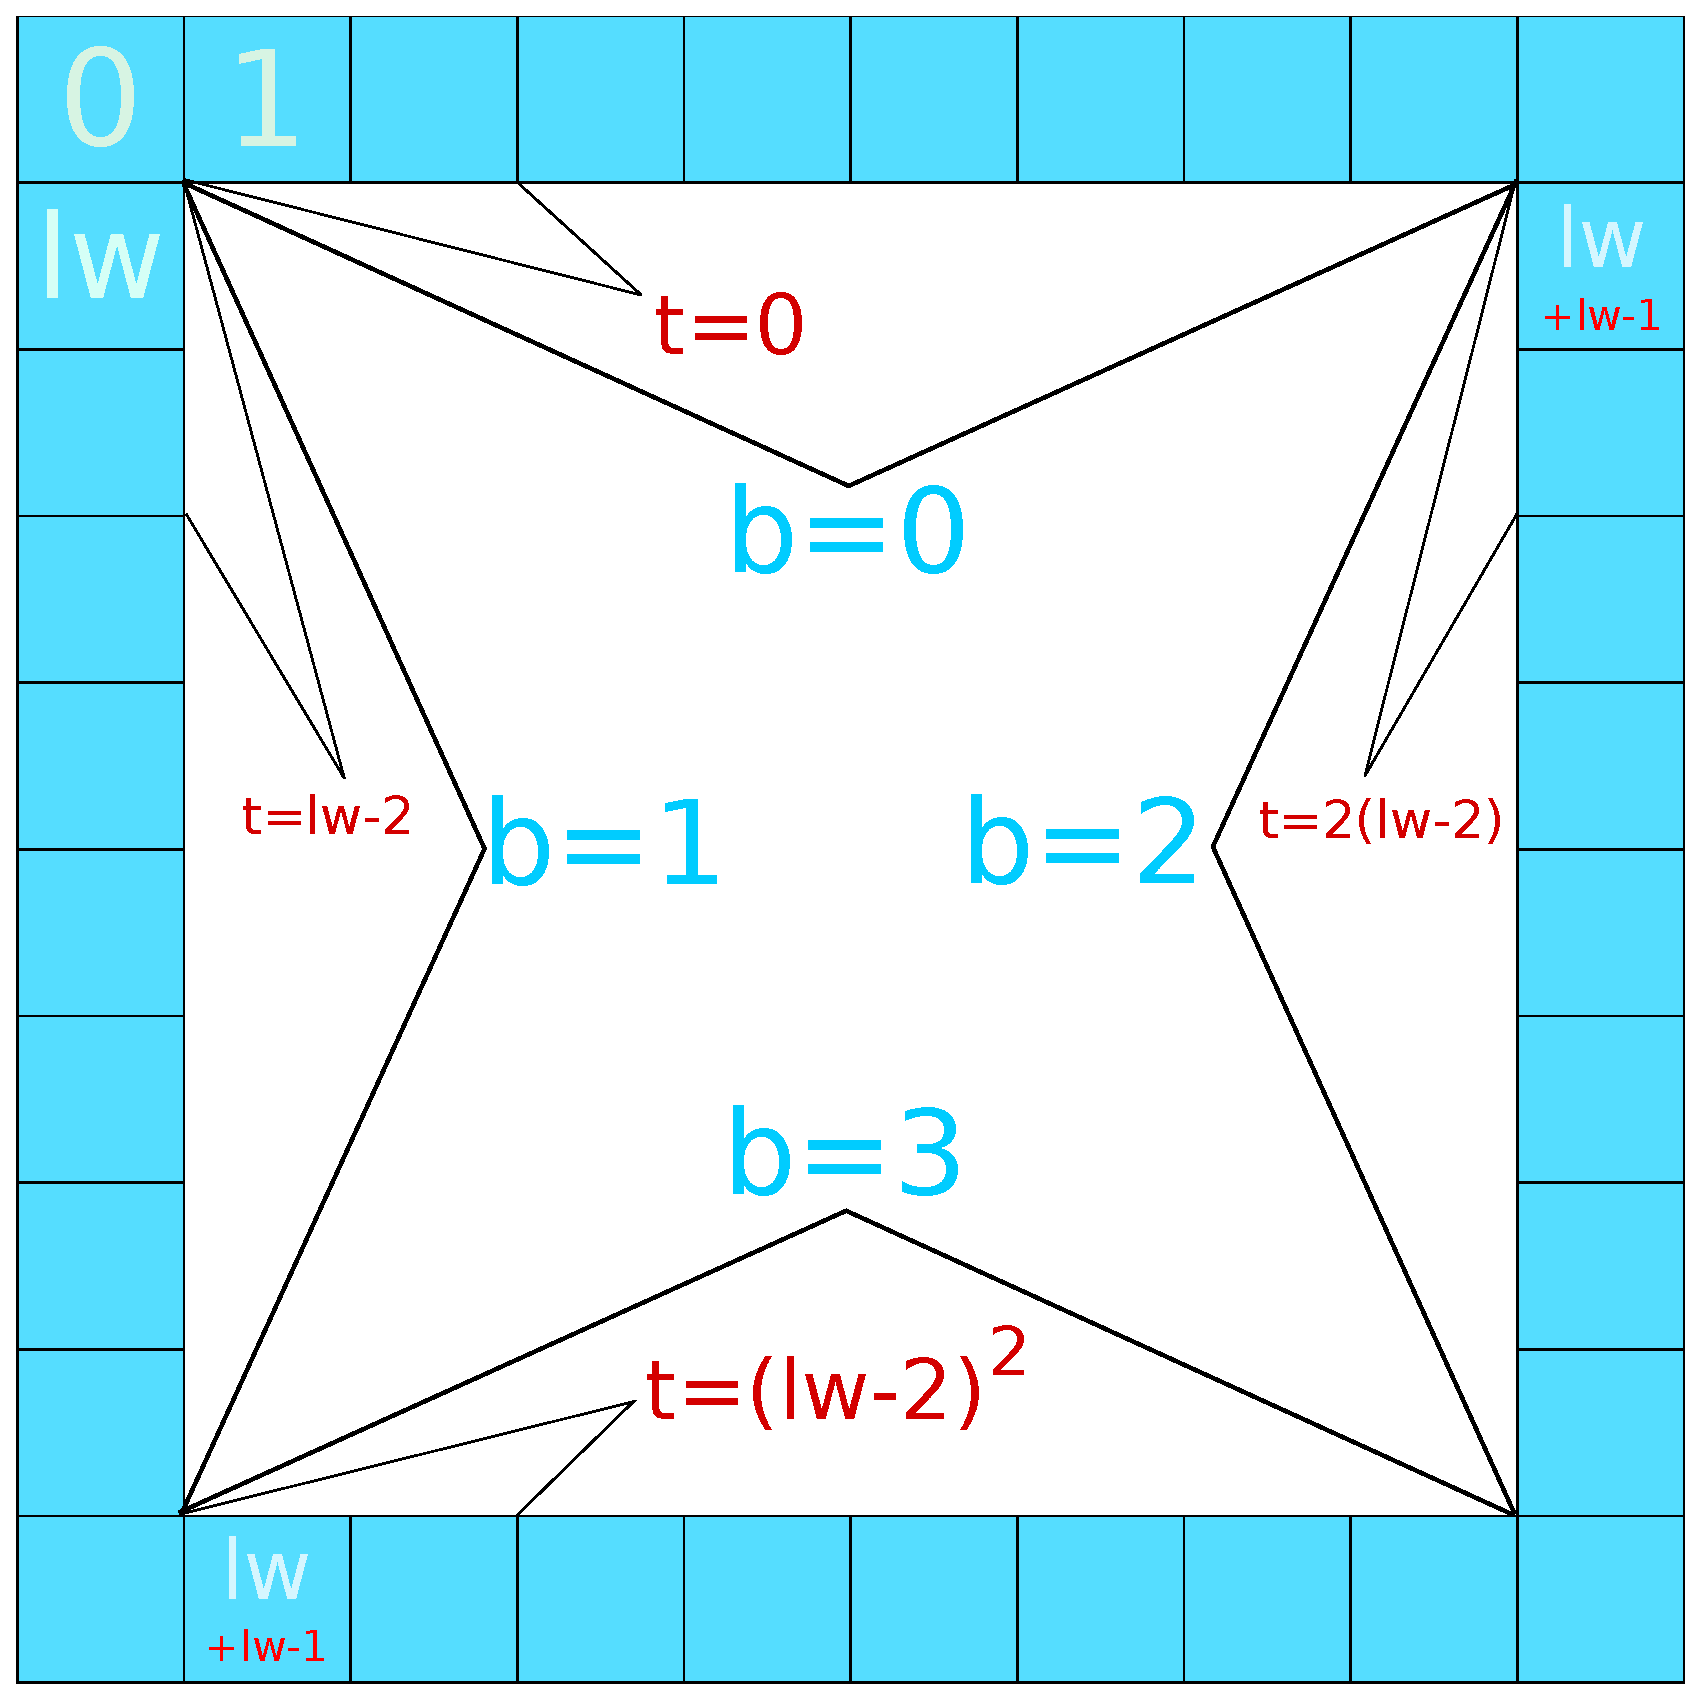
\includegraphics[scale=0.28]{images/borders.eps}
\end{center}
\end{frame}

\begin{frame}[fragile]
\frametitle{integrate2D}
\begin{lstlisting}
for (i = 0; i < consts.n_loop; ++i) {
	T[gid_1d+i] += K[gid_1d_nb+i] *
		(local_T[lid_1d+1+i] + local_T[lid_1d-1+i] 
		+ local_T[lid_1d+lw+i] + local_T[lid_1d-lw+i] 
		- 4*local_T[lid_1d+i])
		
		+ dT[gid_1d_nb+i];
}
\end{lstlisting}
\end{frame}


% Memory
\begin{frame}
\frametitle{Shared Memory}
\framesubtitle{Random errors}
\begin{center}
\includegraphics[scale=0.4]{../check/borders_1c_01.png}
\end{center}
\end{frame}


\begin{frame}
\frametitle{Shared Memory}
\framesubtitle{Synchronized threads}
\begin{center}
\includegraphics[scale=0.4]{../check/borders_sync.png}
\end{center}
\end{frame}

\section{Performances}
\begin{frame}
\frametitle{Stability}
\begin{center}
$\Delta t = 0.001 \longrightarrow \Delta t = 0.002$
\includegraphics[scale=0.27]{../check/stable_001.png}
\includegraphics[scale=0.27]{../check/unstable_002.png}
\end{center}
\end{frame}

\begin{frame}[fragile]
\frametitle{Performances}
\framesubtitle{GPU}
\begin{lstlisting}
Device 0: "GeForce GTX 780"

CUDA Driver Version / Runtime Version          8.0 / 6.5
CUDA Capability Major/Minor version number:    3.5
Total amount of global memory:                 3071 MBytes
(12) Multiprocessors, (192) CUDA Cores/MP:     2304 CUDA Cores
GPU Clock rate:                                941 MHz
Memory Clock rate:                             3004 Mhz
Memory Bus Width:                              384-bit
L2 Cache Size:                                 1572864 bytes

Total amount of constant memory:               65536 bytes
Total amount of shared memory per block:       49152 bytes
Total number of registers available per block: 65536
Warp size:                                     32
Maximum number of threads per multiprocessor:  2048
Maximum number of threads per block:           1024
\end{lstlisting}
\begin{center}

\end{center}
\end{frame}

\begin{frame}
\frametitle{Performances}
\framesubtitle{Execution time}
\begin{center}
\includegraphics[scale=0.5]{../check/time/speed.png}
\end{center}
\end{frame}

\begin{frame}
\frametitle{Performances}
\framesubtitle{Execution time GPU vs CPU}
\begin{center}
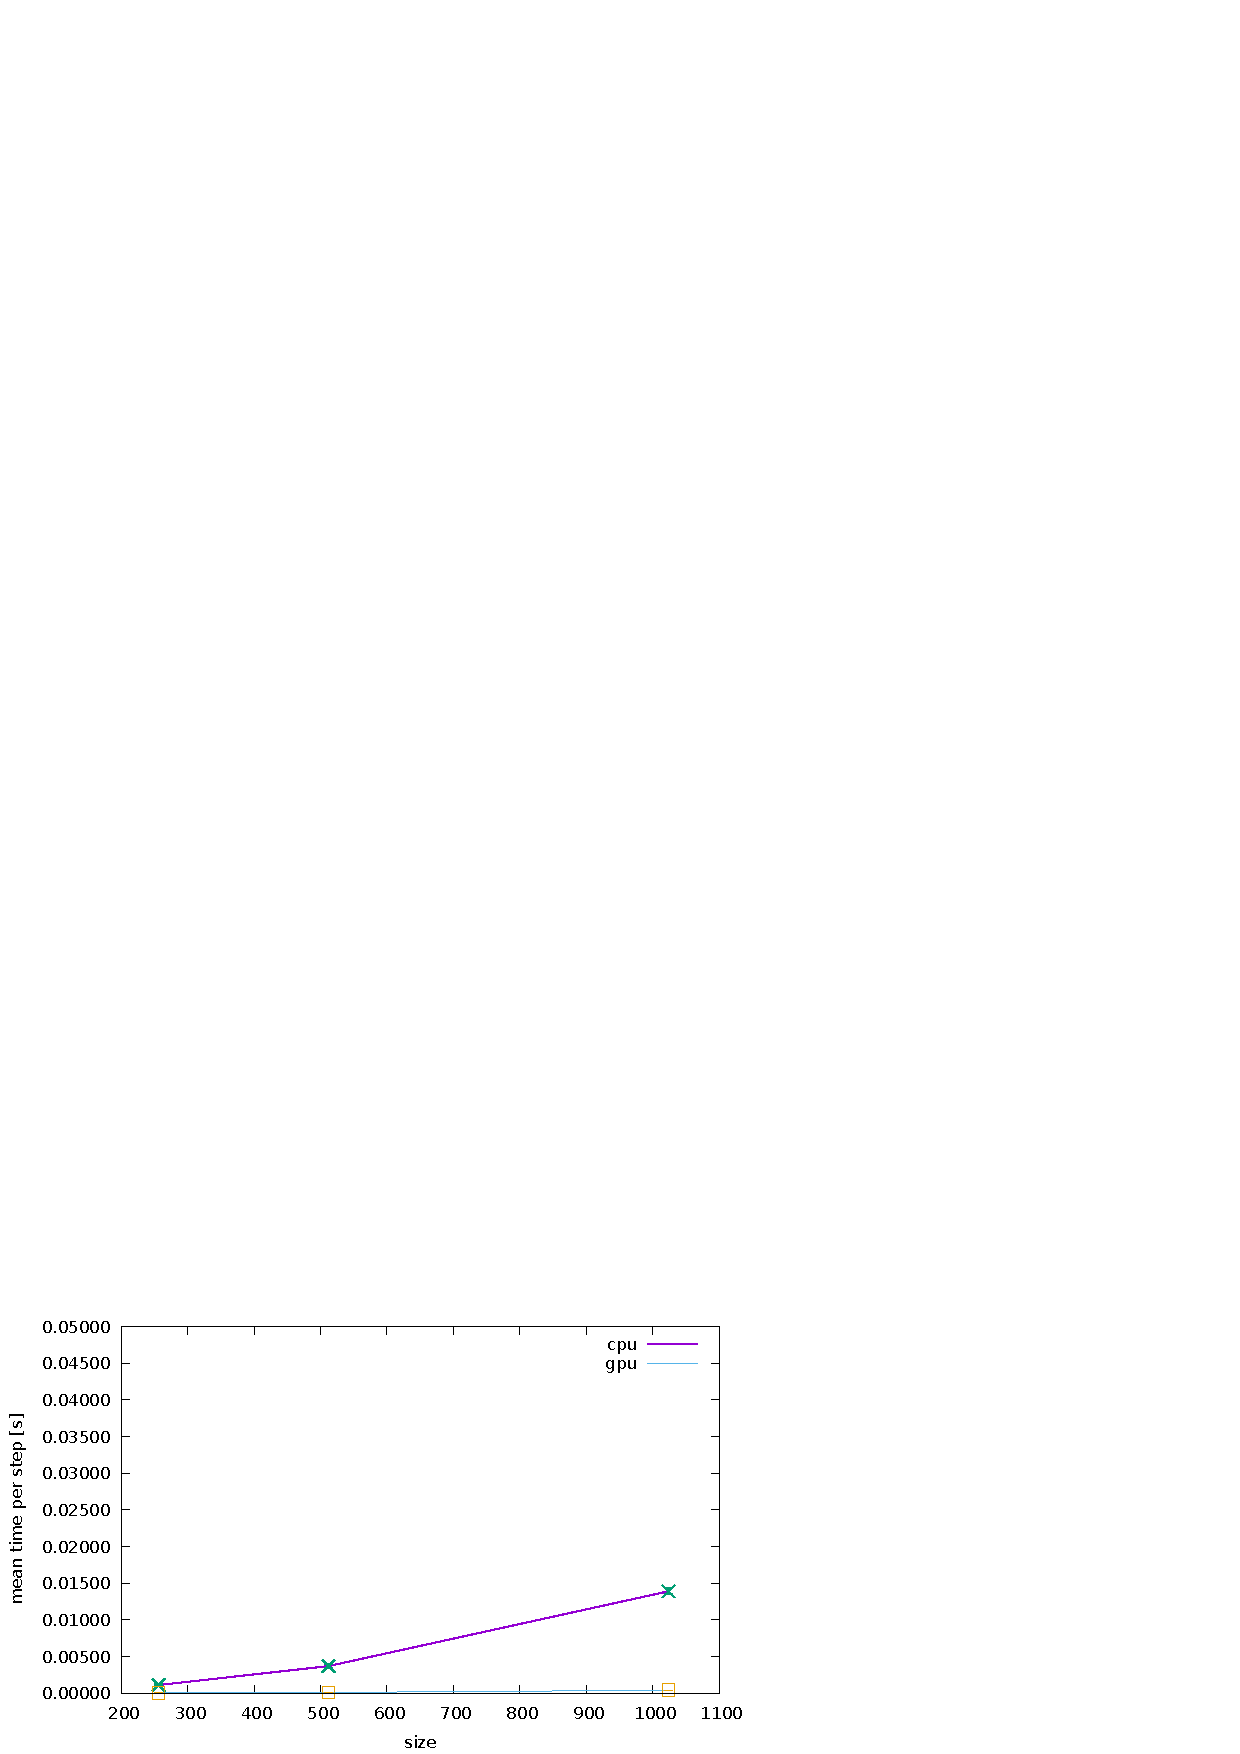
\includegraphics[scale=0.4]{../check/cpu/speed1.png}
\end{center}
\end{frame}

\begin{frame}
\frametitle{Performances}
\framesubtitle{Execution time GPU vs CPU}
\begin{center}
\includegraphics[scale=0.4]{../check/cpu/speed.png}
\end{center}
\end{frame}

\begin{frame}
\frametitle{Performances}
\framesubtitle{Different GPUs}
\begin{center}
\begin{tabular}{l l r}
GeForce GTX 960		&	(sandy1)	&	$8.3\pm0.1\times10^{-5}$ s\\
GeForce GTX 780		&	(sandy2)	&	$8.5\pm0.2\times10^{-5}$ s\\
GeForce GTX 470		&	(seven1)	&	$1.1\pm0.2\times10^{-4}$ s\\
GeForce GTX 560 Ti	&	(seven4)	&	$1.12\pm0.03\times10^{-4}$ s\\
-	&	(seven3)	&	n.w.\\
GeForce 210			&	(seven5)	&	n.w.\\
\end{tabular}
\end{center}
\end{frame}


\section{OpenGL-CUDA interoperability}
\begin{frame}

\frametitle{OpenGL}

OpenGL is a graphics API (similar in scope to Direct3D) that allows to use the
graphics card to draw 2D and 3D vector graphics.

\begin{itemize}
    \item{1992 - OpenGL is first released}
    \item{2004 - OpenGL 2.0 is released. Adds support for programmable pipeline (shaders).}
    \item{2010 - OpenGL 4.0 is released. Adds support for geometry shader (tesselation).}
\end{itemize}

\begin{center}
    \includegraphics[width=\textwidth]{images/pipeline.png}
\end{center}

\end{frame}

% ---------------------------------------------------------------------

\begin{frame}[fragile]

\frametitle{Old method for drawing}

\begin{center}
\begin{lstlisting}
glColor3f(1.0f, 0.0f, 0.0f);
glBegin(GL_QUADS);
    glVertex2f(-0.25f, 0.25f);
    glVertex2f(-0.5f, -0.25f);
    glVertex2f(0.5f, -0.25f);
    glVertex2f(0.25f, 0.25f);
glEnd();
\end{lstlisting}
\end{center}

Moreover the API had to support many features, for example textures coordinates,
lighting, shadows, coordinate transformation and perspective matrices.
\newline
\\
This results in a complex API and lack of flexibility.

\end{frame}

% ---------------------------------------------------------------------

\begin{frame}[fragile]

\frametitle{Modern approach}

\begin{itemize}
    \item{Allow management of GPU memory from host CPU.}
    \item{Programmable pipeline with shaders.}
\end{itemize}

\vspace{5mm}
\textbf{Advantages}: great flexibility, reduced complexity of API and driver implementations
\newline
\\
\textbf{Disadvantages}: lots of boiler-plate code, not noob-friendly

\end{frame}

% ---------------------------------------------------------------------

\begin{frame}[fragile]

\frametitle{OpenGL state machine}

Since the rendering of the 3D scene is a very complex task, OpenGL uses
the concept of state machine to simplify the API interface (avoid function
with too many arguments).

\begin{center}
\begin{lstlisting}
// Tell OpenGL which array contains the data
glBindBuffer(GL_ARRAY_BUFFER, vbo);
// Specify how the data for position can be accessed
glVertexAttribPointer(0, size, GL_FLOAT, GL_FALSE, 0, 0);
// Enable the attribute
glEnableVertexAttribArray(0); // location = 0

// Draw
glDrawArrays(type, 0, vertex_num);
\end{lstlisting}
\end{center}

\end{frame}

% ---------------------------------------------------------------------

\begin{frame}[fragile]

\frametitle{OpenGL VBOs}

VBO (Vertex Buffer Object) - is an array of data in the GPU memory for storing vertices.

\vspace{5mm}

\begin{lstlisting}
GLuint vbo;

// Tell OpenGL we want to allocate array
glGenBuffers(1, &vbo);
/* Tell OpenGL we want to modify the state
    of the following array */
glBindBuffer(GL_ARRAY_BUFFER, vbo);

// Actually allocate memory
glBufferData(GL_ARRAY_BUFFER, size,
    NULL, GL_DYNAMIC_DRAW);

// Tell OpenGl we are done with the array
glBindBuffer(GL_ARRAY_BUFFER, 0);
\end{lstlisting}

\end{frame}

\begin{frame}[fragile]

\frametitle{OpenGL Textures}

Texture - is an image that is mapped to vertices.

\begin{center}
\includegraphics[width=\textwidth]{images/uv.png}
\end{center}

\end{frame}

% ---------------------------------------------------------------------

\begin{frame}[fragile]

\frametitle{OpenGL Textures}

\begin{lstlisting}[basicstyle=\fontsize{7pt}{8pt}\ttfamily]
GLuint texture;

// Tell OpenGl we want to allocate a texture
glGenTextures(1, &texture);
/* Tell OpenGl we are going to modify the state
    of the following texture */
glBindTexture(GL_TEXTURE_2D, texture);

// Set interpolation method to linear
glTexParameteri(GL_TEXTURE_2D, GL_TEXTURE_MIN_FILTER, GL_LINEAR);
glTexParameteri(GL_TEXTURE_2D, GL_TEXTURE_MAG_FILTER, GL_LINEAR);

// Actually allocate memory
glTexImage2D(GL_TEXTURE_2D, 0, GL_RGBA8, width, height,
    0, GL_RGBA, GL_UNSIGNED_BYTE, NULL);    

// Tell OpenGl we finished modifying this etxture
glBindTexture(GL_TEXTURE_2D, 0);
\end{lstlisting}


\end{frame}


% ---------------------------------------------------------------------

\begin{frame}[fragile]

\frametitle{OpenGL shaders}

Shaders \textrightarrow $\,$ programs that run on the GPU (analogous to CUDA kernels).
\newline
\\
Three types:
\begin{itemize}
    \item{Vertex shader - transforms vertex coordinates.}
    \item{Fragment shader - transforms pixel colors.}
    \item{Geometry shader - can add vertices.}
\end{itemize}

\begin{center}
\includegraphics[width=\textwidth]{images/shaders.png}
\end{center}

\end{frame}
% ---------------------------------------------------------------------

\begin{frame}[fragile]

\frametitle{Vertex shader}

\begin{lstlisting}
#version 330

layout(location = 0) in vec2 position;
out vec2 texCoord;

void main() {
    texCoord = vec2(position.x/2 + 0.5, position.y/2 + 0.5);
    gl_Position = vec4(position.x, position.y, 1.0, 1.0);
}
\end{lstlisting}

\end{frame}
% ---------------------------------------------------------------------

\begin{frame}[fragile]

\frametitle{Fragment shader}

\begin{lstlisting}[basicstyle=\fontsize{7pt}{8pt}\ttfamily]
#version 330

uniform sampler2D tex;
in vec2 texCoord;
out vec4 colorOut;

void main() {
    float strength = texture(tex, texCoord).x;

    // Colormap
    //   1     red      (1, 0, 0)
    //   0.75  yellow   (1, 1, 0)
    //   0.5   green    (0, 1, 0)
    //   0.25  cyan     (0, 1, 1)
    //   0     blue     (0, 0, 1)
    // RED
    float red = (strength > 0.75) ?
        1 : ((strength > 0.5) ?
            (strength - 0.5) * 4 : 0);
    // GREEN
    float green = (strength <= 0.75 && strength > 0.25) ?
        1 : ((strength > 0.75) ? 1 - strength : strength) * 4;
    // BLUE
    float blue = (strength > 0.5) ?
        0 : ((strength > 0.25) ?
            (0.5 - strength) * 4 : 1);

    colorOut = vec4(red, green, blue, 1);
}
\end{lstlisting}

\end{frame}
% ---------------------------------------------------------------------

\begin{frame}[fragile]

\frametitle{How to draw}

\begin{lstlisting}
// Select texture unit
glActiveTexture(GL_TEXTURE0);
// Use this texture
glBindTexture(GL_TEXTURE_2D, texture);

// Assign texture unit index to the fragment shader
glUniform1i(1, 0); // location = 1, texture unit = 0

/*** We need a support to draw our texture ***/
// Tell OpenGL which array contains the data
glBindBuffer(GL_ARRAY_BUFFER, vbo);
// Specify how the data for position can be accessed
glVertexAttribPointer(0, 2, GL_FLOAT, GL_FALSE, 0, NULL);
// Enable the attribute
glEnableVertexAttribArray(0); // location = 0

// Draw
glDrawArrays(GL_TRIANGLE_STRIP, 0, 4);

// Disable array and texture
glBindBuffer(GL_ARRAY_BUFFER, 0);
glBindTexture(GL_TEXTURE_2D, 0);
\end{lstlisting}

\end{frame}
% ---------------------------------------------------------------------

\begin{frame}[fragile]

\frametitle{OpenGL-CUDA interperability}

Applications:
\begin{itemize}
    \item{Real-time data visualization.}
    \item{Videogames and 3D application can use CUDA for physics simulation or other computations.}
\end{itemize}

\vspace{5mm}

Further notes:
\begin{itemize}
    \item{Very fast because memory do not need to be transfered out of the GPU.}
    \item{Slower than pure CUDA, because GPU is also used to render data.}
    \item{Not suitable in every situation, e.g. when data needs to be analyzed quantitatively.}
\end{itemize}

\end{frame}
% ---------------------------------------------------------------------

\begin{frame}[fragile]

\frametitle{Execution model}

CUDA kernels and OpenGL run on the same GPU sequentially.

\begin{center}
\includegraphics[width=\textwidth]{images/cuda_gl.png}
\end{center}

V-sync needs to be disabled not to limit execution speed.

\end{frame}
% ---------------------------------------------------------------------

\begin{frame}[fragile]

\frametitle{Registering resources}

OpenGL resources can be written by CUDA (interoperability is one-way).
Need registering before use.

\vspace{5mm}

\begin{lstlisting}
GLuint vbo_gl;
GLuint texture_gl;
struct cudaGraphicsResource *vbo_cuda;
struct cudaGraphicsResource *texture_cuda;

// Register array for use with cuda
cudaGraphicsGLRegisterBuffer(&vbo_cuda, vbo_gl,
	cudaGraphicsMapFlagsWriteDiscard);

// Register texture for use with cuda
cudaGraphicsGLRegisterImage(&texture_cuda, texture_gl,
	GL_TEXTURE_2D, cudaGraphicsMapFlagsWriteDiscard);
\end{lstlisting}

\end{frame}

% ---------------------------------------------------------------------

\begin{frame}[fragile]

\frametitle{Mapping resources}

\vspace{3mm}

When CUDA writes to resources, it needs to map the resource,
to avoid conflicts with OpenGL.

\vspace{2mm}

\begin{lstlisting}
// cudaArray is an opaque object
cudaArray *texture_array;
float *image;

// Enables access from CUDA
cudaGraphicsMapResources(1, &texture_cuda, 0);

// Get pointer of the texture
cudaGraphicsSubResourceGetMappedArray(
	&texture_array, texture_cuda, 0, 0);

/* ... do whatever you want with CUDA on 'image' ... */

/* Copy cuda array to texture position
	NOTE: no transfer between GPU and CPU */
cudaMemcpyToArray(texture_array, 0, 0, image,
	size, cudaMemcpyDeviceToDevice);

// Frees resource for use with OpenGL
cudaGraphicsUnmapResources(1, &texture_cuda, 0);

\end{lstlisting}

\end{frame}


% Brief into to opengl
% Intro
% Advantages - Disadvantages
% Execution model
% Registering and Mapping
% State machine
% Arrays and Textures
% Shaders
% Drawing
% Show code


\section{Conclusions}
%\include{}

\section{References}
\begin{frame}

\frametitle{References}

\begin{itemize}
	\item{\emph{What Every CUDA Programmer Should Know About OpenGL} -
		A outdated but useful introduction to OpenGL integration -
		http://www.nvidia.com/content/gtc/documents/1055\_gtc09.pdf (accessed 15 Jun 2016)}
	\item{\emph{Mixing graphics and compute with multiple GPUs} -
		Another presentation from nVidia about OpenGL interoperability -
		http://on-demand.gputechconf.com/gtc/2012/presentations/S0267B-Mixing-Graphics-and-Compute-with-Multiple-GPUs-Part-B.pdf (accessed 15 Jun 2016)}
	\item{\emph{gl\_cuda\_interop\_pingpong\_st} -
		A good example of interoperability done right -
		https://github.com/nvpro-samples/gl\_cuda\_interop\_pingpong\_st (accessed 15 Jun 2016)}
\end{itemize}

\end{frame}


\end{document} 
